
\subsection{Classical Inequalities}
The purpose of this section is to review and continue developing tools and techniques that we can apply to later proofs.  

% ========================
% Lemma: Integral Identity
% ========================
\begin{tcolorbox}
\begin{lemma}[Integral Identity]
Suppose $X$ is a non-negative RV. It follows that 
    \begin{equation}
    E[X] = \int_{0}^{\infty}P(X > t)dt
    \end{equation}
\end{lemma}
\end{tcolorbox}

\begin{proof}
    Suppose $x \geq 0$ is a non-negative real-valued number. It follows that 
    
    \begin{align*}
        x &= \int_{0}^{x} 1 dt = \int_{0}^{\infty} \mathbbm{1}\{x > t\}dt. 
    \end{align*}
    
    Since the above equality holds for any $x \in \mathbb{R} \geq 0$, the equality holds for any random variable $X$ that is non-negative and real-valued. Therefore, by substituting $X$ for $x$ and taking the expectation of both sides, we obtain 
    
    \begin{align*}
        X &= \int_{0}^{X} 1 dt = \int_{0}^{\infty} \mathbbm{1}\{X > t\}dt && \\
        \implies E[X] &= E\left[\int_{0}^{\infty} \mathbbm{1}\{X > t\}dt\right] && \\ 
        &= \int_{0}^{\infty} E\left[\mathbbm{1}\{X > t\}\right]dt &&\text{Fubini-Tonelli} \\
        &= \int_{0}^{\infty} P(X > t) dt && \\ 
    \end{align*}
\end{proof}

\begin{tcolorbox}
\begin{lemma}[Integral Identity (Extension)]
Suppose $X$ is a RV. It follows that 
    \begin{equation}
    E[X] = \int_{0}^{\infty}P(X>t)dt - \int_{-\infty}^{0}P(X < t)dt.
    \end{equation}
\end{lemma}
\end{tcolorbox}

\begin{proof}
Suppose $x\in \mathbb{R}$. We observe that 
    \[ x = 
    \begin{cases}
        \displaystyle{-\int_{-\infty}^{0} \mathbbm{1}\{t > x\} dt} &, x < 0 \\
        \displaystyle{\int_{0}^{\infty} \mathbbm{1}\{t < x\} dt} &, x \geq 0 
    \end{cases}
    \] 
Furthermore, since one of the integrals will be 0, we have  
    \begin{align*}
    x &= \int_{0}^{\infty} \mathbbm{1}\{x>t\}dt - \int_{-\infty}^{0}\mathbbm{1}\{x<t\}dt \\
    X &= \int_{0}^{\infty} \mathbbm{1}\{X>t\}dt - \int_{-\infty}^{0}\mathbbm{1}\{X<t\}dt && \text{Allow $x$ to be a RV}\\
    \implies E[X] &= E\left[\int_{0}^{\infty} \mathbbm{1}\{X>t\}dt\right] - E\left[\int_{-\infty}^{0}\mathbbm{1}\{X<t\}dt\right] && \text{Take expectation}\\
    E[X] &= \int_{0}^{\infty} E\left[\mathbbm{1}\{X>t\}dt\right] - \int_{-\infty}^{0}E\left[\mathbbm{1}\{X<t\}dt\right] && \text{Fubini-Tonelli}\\
    &= \int_{0}^{\infty} P(X > t)dt - \int_{-\infty}^{0}P(X<t)dt 
    \end{align*}
\end{proof}

% ================================
% Proposition: Markov's Inequality
% ================================
\begin{tcolorbox}
\begin{proposition}[Markov's Inequality]
For any non-negative RV, $X$, and $t>0$, 
    \begin{equation}
    P(X \geq t) \leq \frac{E[X]}{t}
    \end{equation}
\end{proposition}
\end{tcolorbox}

\begin{proof}
\begin{align*}
    E[X] &= \int_{0}^{\infty} xp(x)dx && \text{defn. of expectation} \\ 
    &= \int_{0}^{t} xp(x)dx + \int_{t}^{\infty}xp(x)dx && \text{separate integral} \\
    \implies E[X] &\geq \qquad \qquad \qquad \int_{t}^{\infty}xp(x)dx && \text{since $\int_{0}^{t}xp(x)dx \geq 0$} \\
    &\geq \qquad \qquad \qquad \int_{t}^{\infty} tp(x)dx &&\text{since $x \geq t$ in the integral} \\ 
    &= \qquad \qquad \qquad t \int_{t}^{\infty}p(x)dx && \text{since we're not integrating over $t$} \\ 
    &= \qquad \qquad \qquad t P(X \geq t)  \\
    \implies P(X \geq t) &\leq \frac{E[X]}{t}
\end{align*}
\end{proof}


% ===================================
% Proposition: Chebyshev's Inequality
% ===================================
\begin{tcolorbox}
\begin{proposition}[Chebyshev's Inequality]
Suppose $X$ has a finite mean and variance. It follows that 
    \begin{equation}
    P(|X-\mu| \geq t) \leq \frac{\sigma^2}{t^2}
    \end{equation}
\end{proposition}
\end{tcolorbox}

\begin{figure}[H]
    \centering
    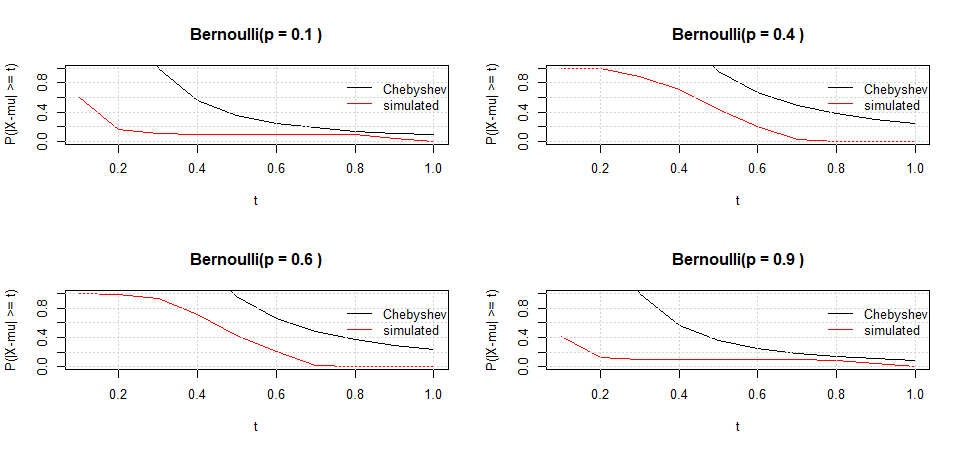
\includegraphics[scale=0.7]{Chebyshev.png}
    \caption{Simulations for Chebyshev's Inequality. We see that the Chebyshev inequality is actually conservative for small $t$, but becomes better as $t$ increases. }
    \label{fig:chebyshev_sim}
\end{figure}
\begin{figure}[H]
    \centering
    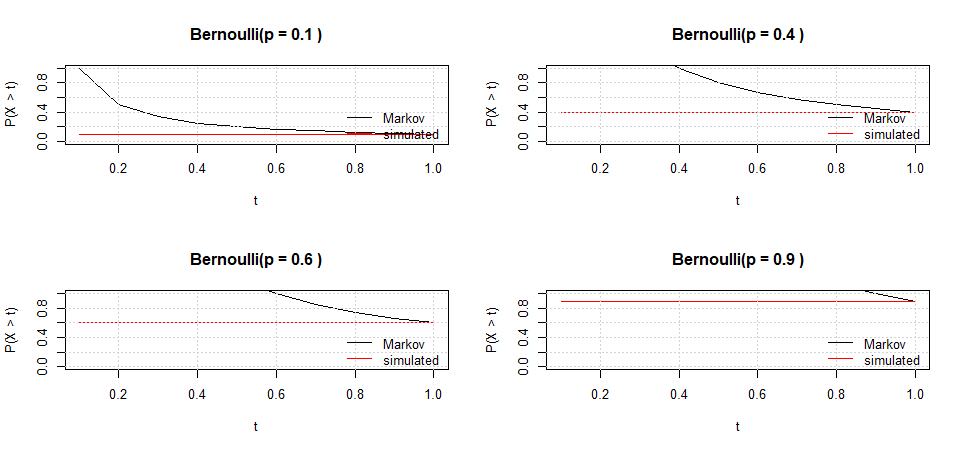
\includegraphics[scale=0.7]{Markov.png}
    \caption{Simulations for Markov's Inequality. Similar to Chebyshev's inequality, the inequality improves for larger $t$. However, the simulated value is constant.}
    \label{fig:markov_sim}
\end{figure}


